\chapter{System test results}
The power supply system was implemented successfully as can be seen in Figure \ref{fig:full_circuit}, all of the sub circuits were tested under various circumstances and passed all of the design requirements, with all of the crucial system measurements tabulated in Table \ref{tab:powersupplytable}. The layout of the chosen positions of the capacitors and inductors caused minimal electromagnetic interference between the components and this meant that all recorded noise measurements were within tolerance.


 \begin{figure}
    \centering
    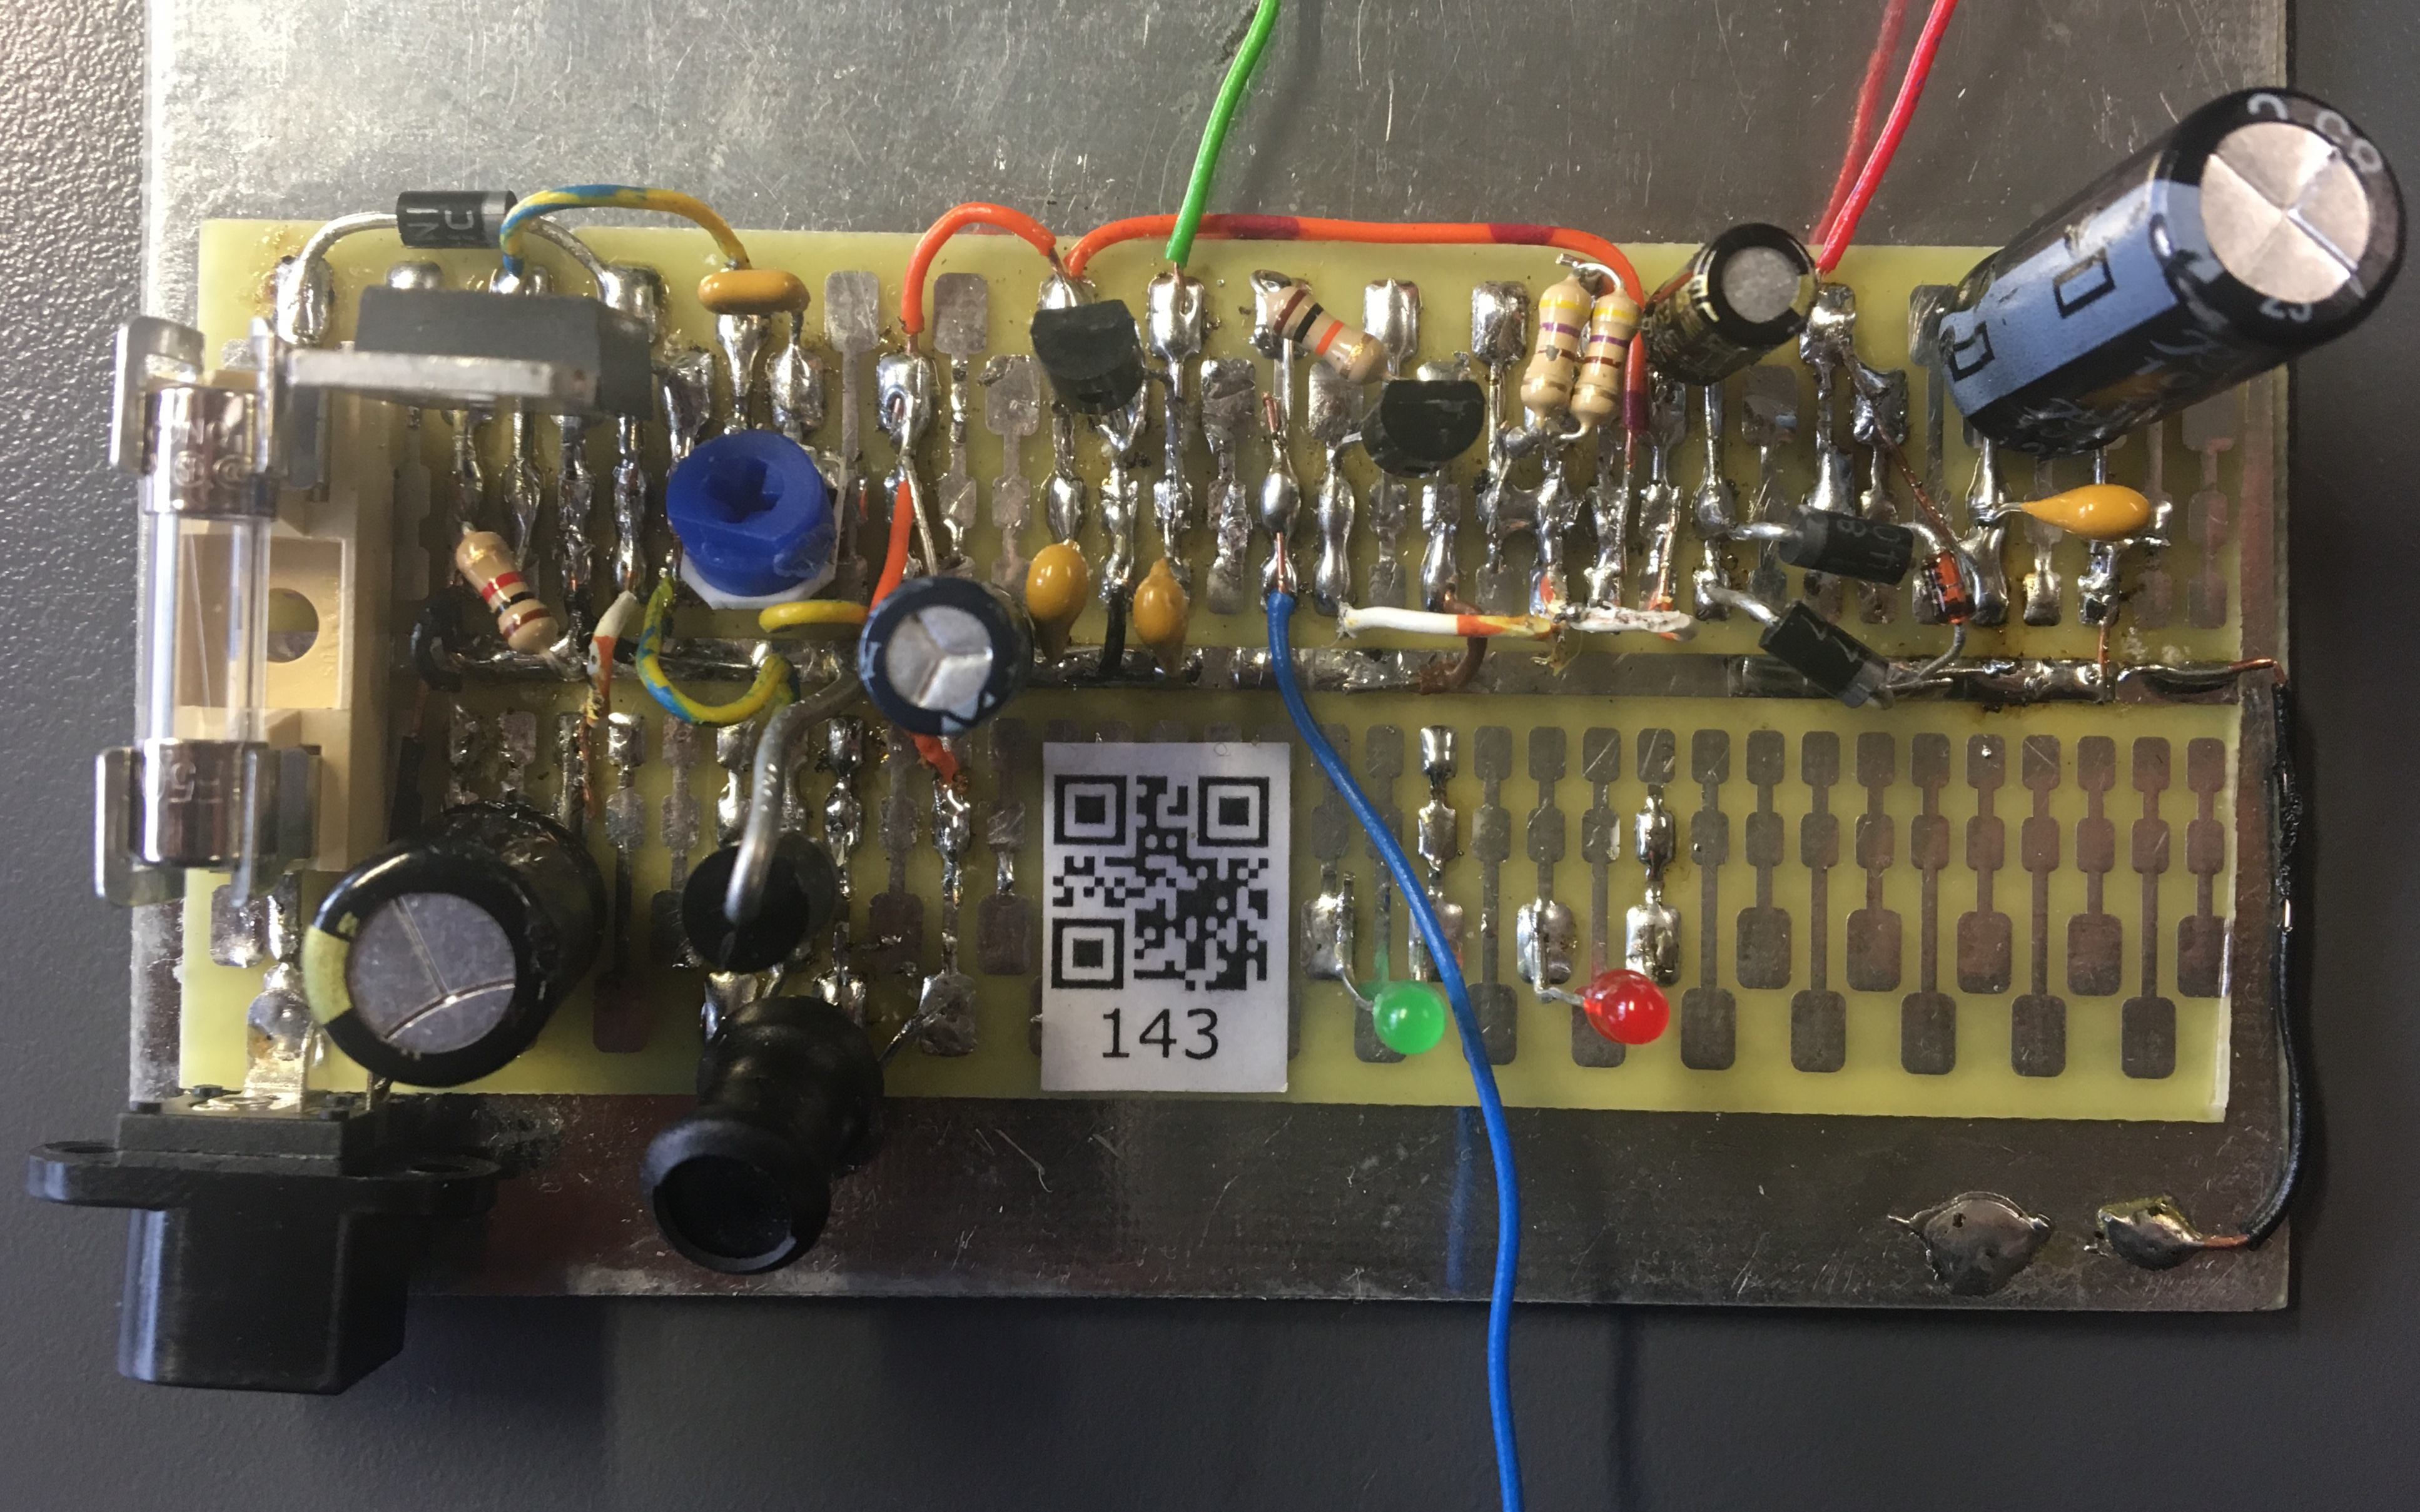
\includegraphics[width = 0.6\linewidth]{Figures/full_circuit.jpg}
    \caption{Full Power Supply Implementation}
    \label{fig:full_circuit}
\end{figure}

\begin{table}
        \centering
        \footnotesize
        \caption{Table Showing Output Characteristics Of Power Supply Subcircuits.}
         \begin{tabular}{c@{\qquad}rrrr}
          \toprule
           Power Supply & Output Voltage ($\SI{}{V}$) & RMS Noise ($\SI{}{mV}$) & Measured Noise ($\SI{}{mV_{pp}}$)\\
           \midrule
            Switch Mode Power Supply & 11.81    & 15.3      & 60.8  \\
            Linear Regulator         & 5.08     & 0.786     & 4.88  \\
            Charge Pump              & -5.00    & 0.175     & 3.44 \\
          \bottomrule
        \end{tabular}
     \label{tab:powersupplytable}
\end{table}





